\section{Motivating Scenario}
%\subsection{Motivating Scenario}
\label{sec:motivation}

\begin{figure*}[ht!]
  \begin{center}
%    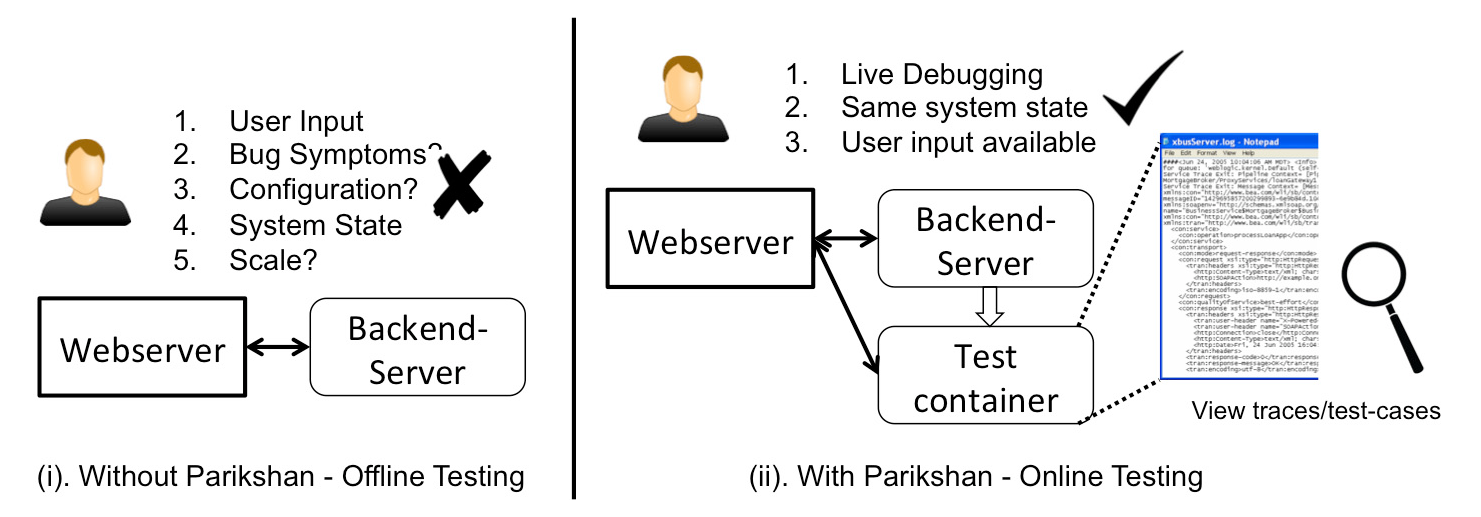
\includegraphics[width=0.7\textwidth]{figs/motivation.eps}
    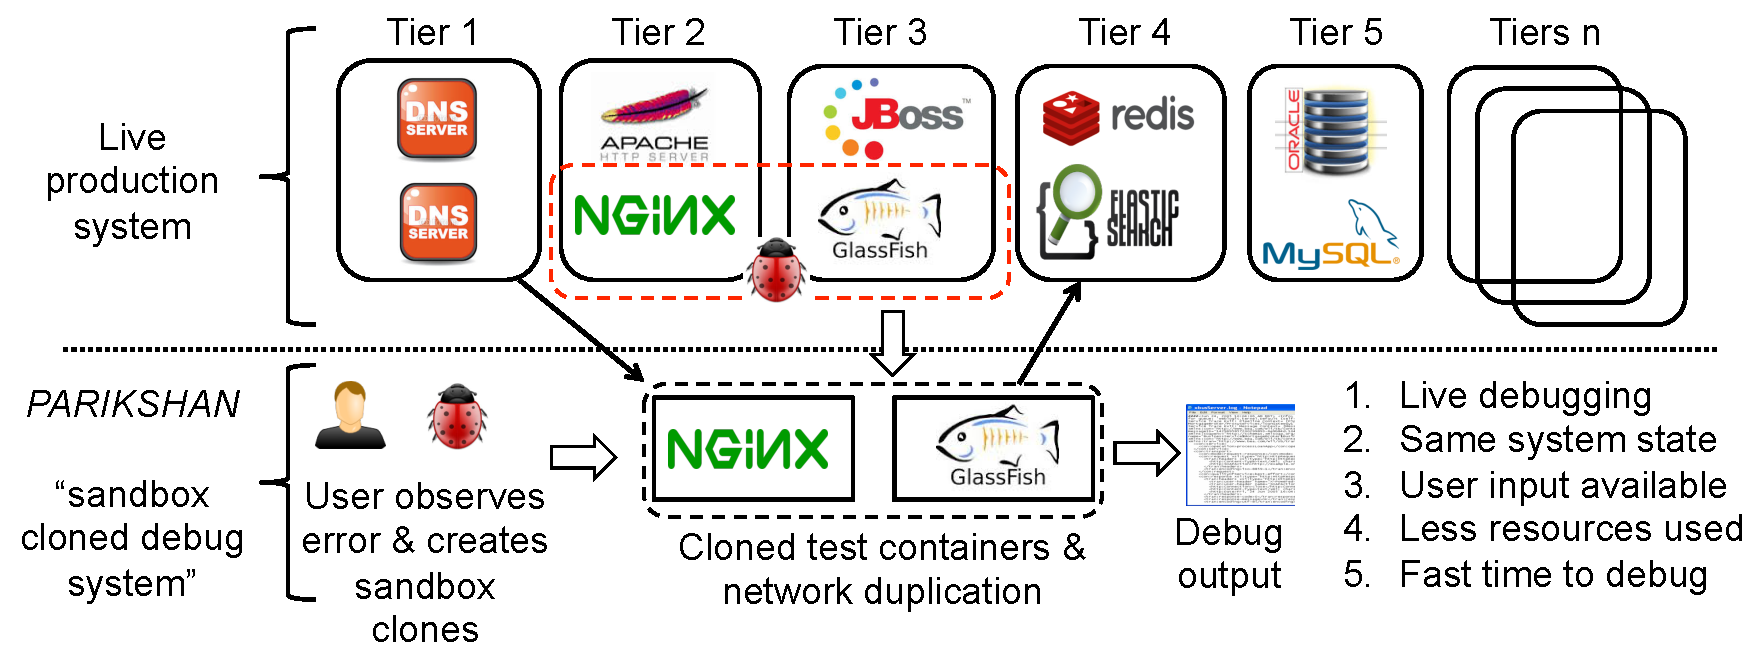
\includegraphics[width=0.95\textwidth]{figs/workflow3.pdf}
    \caption{Workflow of \parikshan in a live multi-tier production system with several interacting services. When the administrator of the system observes errors in two of it's tiers, he can create a sandboxed clone of these tiers and observe/debug them in a sandbox environment without impacting the actual production system.}
    \label{fig:motivation}
  \end{center}
\end{figure*}

\noindent
As a motivating scenario, let us take a complex multi-tier service-oriented system (Figure \ref{fig:motivation}), with several interacting services (web-servers, application servers, search and indexing, database etc.). 
The system is maintained by an operator, who can observe the health of the system using light-weight monitoring, which is part of the deployed system.
In the interest of application performance, production system monitoring is usually limited to system resource usage, application usage statistics, transaction logs, and error logs.

At a certain time in the execution of the system, the operator observes unusual memory usage in the glassfish application server, and some error logs being generated in the nginx web-server. 
He surmises, that there is a potential memory leak/allocation problem in the app-server, or a problem in the web-server.
However, with a limited amount of monitoring information, he can only go so far.

\iffalse
user Joe who is an administrator for a multi-tiered system (see Figure \ref{fig:motivation}). 
Much like several administrators, Joe uses light-weight system instrumentation to get a high level statistical/health view of the system.
He observes an unusually high memory usage in the glassfish server for transaction type X, and some anomalous error logs in the associated nginx systems.
Under usual circumstances, the system would have to go down(depending on the severity of the problem), the problem debugged using offline analysis, and the system would be patched once the problem has been diagnosed. 
However often, it is difficult to find out the configuration of the system, and the user input which is causing this problem.
In modern large scale systems some errors may happen only at scale, and would require a large test-cluster to recreate the error.
Furthermore, taking down the glassfish and nginx servers would impact several more services otherwise are running fine. 
\fi

Typically, trouble tickets are generated for such problems, and they are debugged offline.
However using \parikshan, the operator can fork off clones of the nginx and glassfish containers as \textbf{\textit{nginx-debug}} and \textbf{\textit{glassfish-debug}}.
%Our proxy network duplication now sends a copy of the incoming request to the debug containers, while users can continue using nginx and glassfish services. 
Our network duplication mechanisms ensure that the debug containers receive the same inputs as the production containers, and that the production containers continue to provide service without interruption.
This separation of the production and debug environment, allows the operator to use dynamic instrumentation tools to perform deeper diagnosis without fear of additional disruptions due to debugging.
Since the system has been cloned from the original potentially ``buggy'' production container, it will also exhibit the same memory leaks/or logical errors.
Additionally, \parikshan can focus on the ``buggy'' parts of the system, without needing to replicate the entire system in a test-cluster.
This process will greatly reduce the time to bug resolution, and allow real-time bug diagnosis capability.
%Time to bug resolution is usually a very important criteria in any user-facing service oriented application.
%This , while allowing real-time-diagnosis, significantly reduce the time to bug resolution.

% This paragraph needs serious revision - the points have been noted down but they need to be stated clearly in a better manner.
%One of the key advantages of such an online approach is a reduced time to bug resolution. 
%Time to bug resolution is usually a very important criteria in any user-facing service oriented application, as the longer a bug remains the system, the more it is going to hit the user perception/revenue.
%Bearing this in my mind we believe, that online testing will be an important aspect towards modern applications.
%Additionally the usage of redundant computing for testing in A/B testing(see section \ref{sec:related}) approaches is a well accepted paradigm in real-world applications.
%This leads us to believe that using redundant computing will be acceptable for regular testing approaches as well.
%Using \parikshan is also a way to avoid creating a large test-cluster to do debugging. 

\iffalse
\subsection{Motivation Questions?}

To further motivate our testing paradigm we have come up with a set of motivating questions:

%\begin{compactitem}
%\setlength{\itemsep}{1Pt}
%\item[]\textbf{Q1:} Is it important to sandbox test-cases?
%\item[]\textbf{Q2:} Is recreating production environment difficult? 
%\item[]\textbf{Q3:} Is redundant computing available? 
%\item[]\textbf{Q4:} How would executing test-cases in a production server effect user-experience?
%\end{compactitem}

\subsubsection{\textbf{Q1:} Is it persistent testing important?}
\subsubsection{\textbf{Q2:} Is recreating production environment difficult?}
\subsubsection{\textbf{Q3:} Can redundant computing be utilized for testing?}
\subsubsection{\textbf{Q4:} How would executing test-cases in a production server effect user-experience?}
\fi